%
\documentclass[%
 reprint,
 amsmath,amssymb,
 aps,
]{revtex4-1}

\usepackage{graphicx}% Include figure files
\usepackage{dcolumn}% Align table columns on decimal point
\usepackage{bm}% bold math


\begin{document}

\begin{titlepage}
\begin{center}
\large{UNIVERSIDAD PRIVADA DE TACNA}\\
\vspace*{-0.025in}
\begin{figure}[htb]
\begin{center}

\includegraphics[width=8cm]{./Imagenes/upt}
\end{center}
\end{figure}
\vspace*{0.15in}
INGENIERIA DE SISTEMAS  \\

\vspace*{0.5in}
\begin{large}
TITULO:\\
\end{large}

\vspace*{0.1in}
\begin{Large}
\textbf{Trabajo Fina de l Unidad III} \\
\end{Large}

\vspace*{0.3in}
\begin{Large}
\textbf{CURSO:} \\
\end{Large}

\vspace*{0.1in}
\begin{large}
BASE DE DATOS II\\
\end{large}

\vspace*{0.3in}
\begin{Large}
\textbf{DOCENTE(ING):} \\
\end{Large}

\vspace*{0.1in}
\begin{large}
 Patrick Cuadros Quiroga\\
\end{large}

\vspace*{0.2in}
\vspace*{0.1in}
\begin{large}
Integrantes: \\
\begin{flushleft}
Adnner Esperilla Ruiz		\hfill	(2015050543) \\
Wilfredo Vilca Chambilla		\hfill	(2006028540) \\
\vspace*{0.5in}
\begin{center}
2019-Tacna\\
\end{center}
\vspace*{1.5in}
\end{flushleft}
\end{large}
\end{center}

\end{titlepage}


\title{Estrategias de seguridad en base de datos}


\begin{abstract}
\begin{center}
\textbf{Resumen}
\end{center}
El mundo de la informática es vulnerable de sufrir algún tipo de ataque por terceras personas, con la
intención de propagar algún tipo de malware o robar información importante de la víctima. Por todo esto,
es fundamental tomar las medidas que sean necesarias para mantener a buen recaudo la información.
\par Dentro de todo esto, las bases de datos son uno de los sistemas que más sufren este tipo de ataques, en
gran medida a que es ahí donde en la mayoría de las ocasiones está almacenada la información. Para
acceder a ella, los hackers buscan cualquier tipo de vulnerabilidad que no haya sido controlada para
acceder al sistema y hacerse con aquello que les sea de interés.

\textbf{Palabras clave:}   virtualizacion, contenedores, simulacion, procesos\\

\begin{center}
\textbf{Abstract}
\end{center}

The computer world is vulnerable to suffer some type of attack by third parties, with the
intention to spread some type of malware or steal important information from the victim. For all this,
It is essential to take the necessary measures to keep the information safe.
 \par Within all this, the databases are one of the systems that suffer most from this type of attacks, in
great extent to that is where, in most cases, information is stored. For
access it, hackers look for any type of vulnerability that has not been controlled for
access the system and get what is of interest.
\textbf{Keywords:}   virtualization, containers, simulation, resources.\\

\end{abstract}



\maketitle

%\tableofcontents

\section {Introducción}\label{sec:1}





%-----------------------------------------------------------------
\section{Objetivos}\label{sec:2}
\subsection{General:}
-  Poder diferenciar y sacar caracteristicas principales  en las maquinas virtuales contendedores .
\subsection{Específicos:}
-  Definir los conceptos de maquinas virtuales y contenedores.\\
- Comparar las caracteristicas principales.

%-----------------------------------------------------------------
\section {Marco Teórico}

\subsection{¿Qué es seguridad de base de datos?}

%-------------------------------------------------

\subsection{Principios básicos de la seguridad de base de datos}
\begin{itemize}
	\item \textbf{Identifique su sensibilidad: }Una cosa hay que tener claro, y es que no se puede asegurar aquello que no se conoce. Con esto queremos
decir que es importante conocer la sensibilidad de nuestro sistema de bases de datos para saber cómo
actuar y mejorar de esta forma su seguridad. Para ello podemos hacer uso de herramientas de
identificación que nos ayuden a encontrar posibles agujeros por donde podríamos ser atacados.

	\item \textbf{Evaluación de la vulnerabilidad y la configuración:} Evalúe la configuración de tu base de datos para descartar posibles agujeros de seguridad. Esto incluye la
verificación de la forma en la que ésta fue instalada y la de tu sistema operativo. Por ejemplo podríamos
verificar los privilegios de los distintos grupos de usuarios respecto a las acciones de ejecutar, leer y escribir
en bases de datos.

	\item \textbf{Endurecimiento: }Como resultado de una evaluación de la vulnerabilidad a menudo se dan una serie de recomendaciones específicas. Este es el primer paso en el endurecimiento de la base de datos. Otros elementos de endurecimiento implican la eliminación de todas las funciones y opciones que se no utilicen. Aplique una política estricta sobre que se puede y que no se puede hacer, pero asegúrese de desactivar lo que no necesita.
	\item \textbf{Audite: }Una vez que hayamos creado una configuración que creamos que puede ser totalmente segura, realicemos
actividades de auditoría para asegurarnos que no te desvías de tu objetivo. Por ejemplo, se podría poner
algún tipo de alarma para que nos avisara de cualquier cambio que se pudiera dar en dicha configuración.
	\item \textbf{Monitoreo:} Monitorizar la actividad que se lleva a cabo en nuestra base de datos nos puede dar algún tipo de pista en
caso de estar siendo utilizada de forma indebida o para la detección de intrusos.
El monitoreo dinámico es también un elemento esencial de la evaluación de vulnerabilidad, le permite ir más allá de evaluaciones estáticas o forenses. Un ejemplo clásico lo vemos cuando múltiples usuarios comparten credenciales con privilegios o un número excesivo de inicios de sesión de base de datos.
	\item \textbf{Pistas de Auditoría: }Aplique pistas de auditoría y genere trazabilidad de las actividades que afectan la integridad de los datos, o la visualización los datos sensibles.
Recuerde que es un requisito de auditoría, y también es importante para las investigaciones forenses.
La mayoría de las organizaciones en la actualidad emplean alguna forma de manual de auditoría de transacciones o aplicaciones nativas de los sistemas gestores de bases de datos. 
	\item \textbf{ Control de acceso y Gestión de derechos: }No todos los datos son igual de importantes y no todos los usuarios son creados igual. Es necesario
establecer una jerarquía y garantizar que cada tipo de usuario sólo pueda realizar las acciones que se le
permiten en la base de datos, para garantizar de esa forma la integridad de la información.
\par En el caso de los datos confidenciales, como pueden ser todo tipo de contraseñas, es recomendable utilizar
algún tipo de cifrado de datos para que la información no sea legible a simple vista.
\par  En este White Paper hemos visto las principales vulnerabilidades que nos podemos encontrar sobre las
bases de datos, vulnerabilidades que nos pueden dar más de un quebradero de cabeza si no tomamos las
medidas necesarias para paliarlas. \cite{ff}

\end{itemize}

%-------------------------------------------------

\subsection{Medidas de seguridad y tipos de la seguridad de base de datos}
Las medidas de seguridad a considerar son las siguientes: 
\begin{itemize}
	\item \textbf{Físicas: }Viene a ser un control quienes tienen acceso al equipo
	\item \textbf{Personal: }Se da los permisos al personal autorizado 
	\item \textbf{Sistema Operativo: }Elegir tu Sistema Operativo que daran seguridad a tu informacion
	\item \textbf{SGBD: }Utilizar algunas herramientas que dara facilidad el SGBD
\end{itemize}
Existen dos tipos de mecanismos de seguridad de base de datos:
\begin{itemize}
	\item \textbf{Discrecional: }Se usan para otorgar permisos  a los usuarios, incluida la capacidad de tener acceso a archivos, registros o campos de datos específicos en un determinado modo.
	\item \textbf{Obligatoria: }Sirven para imponer igualdad de múltiples niveles clasificando los datos y los usuarios en varias clases (o niveles) de seguridad e implementando después la política de seguridad apropiada de la organización.
	\item Otra técnica de seguridad es el  \textbf{Encriptado de datos}, que sirven para proteger datos confidenciales que se transmiten  por algún otro tipo de red de comunicaciones. El cifrado puede proveer protección adicional a secciones confidenciales de una base de datos \cite{l}
\end{itemize}
%-------------------------------------------------

\subsection{Requisitos para la seguridad de base de datos}
Para mantener la seguridad de la base de datos se necesita establecer controles para la protejan de futuros ataques extrenos, caídas o fallos del software o del equipo. Por ello, aquí se nombrará requisitos para tener un buen control de la seguridad de datos.
\begin{itemize}
\item La base de datos debe ser protegida contra el fuego, el robo y otras
formas de destrucción.
\item Los datos deben ser reconstruibles, ya que siempre pueden ocurrir
accidentes.
\item Los datos deben poder ser sometidos a procesos de auditoria.
\item El sistema debe diseñarse a prueba de intromisiones, no deben
poder pasar por alto los controles.
\item Ningún sistema puede evitar las intromisiones malintencionadas,
pero es posible hacer que resulte muy difícil eludir los controles.
\item El sistema debe tener capacidad para verificar que sus acciones han
sido autorizadas.
\item Las acciones de los usuarios deben ser supervisadas, de modo tal
que pueda descubrirse cualquier acción indebida o errónea. \cite{book1}
\end{itemize}
%-------------------------------------------------

\subsection{Características de la seguridad de base de datos}
El objetivo es proteger la base de datos contra los accesos no autorizados.
\begin{itemize}
\item \textbf{Confidencialidad de la informacion :} Se trata de la característica más importante de la seguridad de base de datos. Se logra a través del La encriptación que ha de aplicarse a datos en reposo, pero también a los datos que, por un motivo u otro, se encuentren en tránsito. \\ Por tanto, unicamente las personas que tengan la autorización correspondiete pueden acceder a la información almacenada.
\item \textbf{Integridad de la informacion:}La integridad de la base de datos se refiere a la validez y la consistencia de los datos almacenados. Normalmente, la integridad se expresa mediante restricciones o reglas que no se pueden violar. Estas restricciones se pueden aplicar tanto a los datos, como a sus relaciones, y es el SGBD quien se debe encargar de mantenerlas.
\begin{center}
	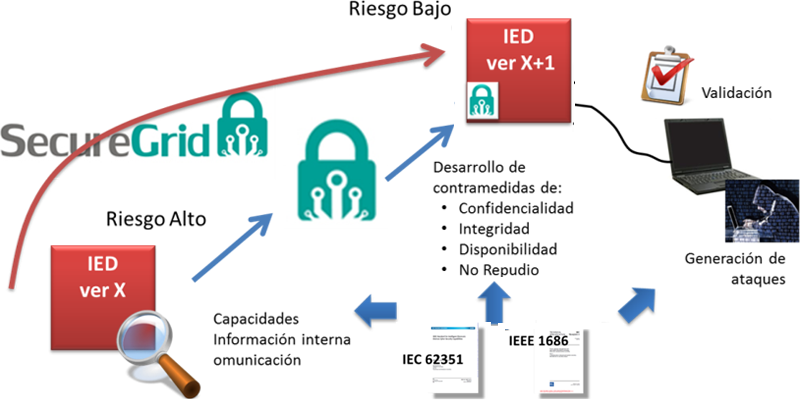
\includegraphics[width=9cm]{./Imagenes/integridad}
\end{center}	
\item \textbf{Disponibilidad de la informacion:} La información debe estar disponible para todos los usuarios con autorización en el momento que requieran.
\item \textbf{Seguridad de la informacion:} La seguridad de la base de datos es la protección de la base de datos frente a usuarios no autorizados. Sin unas buenas medidas de seguridad, la integración de datos en los sistemas de bases de datos hace que éstos sean más vulnerables que en los sistemas de ficheros.
\item \textbf{Concurrencia:}En algunos sistemas de ficheros, si hay varios usuarios que pueden acceder simultáneamente a un mismo fichero, es posible que el acceso interfiera entre ellos de modo que se pierda información o se pierda la integridad. La mayoría de los SGBD gestionan el acceso concurrente a la base de datos y garantizan que no ocurran problemas de este tipo.
\item \textbf{Recuperación:}Muchos sistemas de ficheros dejan que sea el usuario quien proporcione las medidas necesarias para proteger los datos ante fallos en el sistema o en las aplicaciones. Los usuarios tienen que hacer copias de seguridad cada día, y si se produce algún fallo, utilizar estas copias para restaurarlos. \cite{web1}

\end{itemize}
\begin{center}
	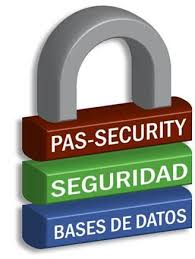
\includegraphics[width=7cm]{./Imagenes/imagen1}
\end{center}	
Garantizar la integridad en base de datos, así como su disponibilidad y confiabilidad es determinante para el buen funcionamiento del negocio. Sin embargo, la amenaza no da tregua y, a día de hoy, los ataques se multiplican, tanto en frecuencia, como en objetivo. \\\\  Los piratas informáticos ya no codician sólo los activos informacionales de las grandes corporaciones multinacionales, sino que tienen en su punto de mira a todo tipo de empresas, independientemente de su tamaño, propósito o industria.
%-------------------------------------------------


\subsection{Importancia de la seguridad de base de datos}
\begin{itemize}
	\item Es importante desarrollar una política de seguridad para cada base de datos. La política de seguridad establece métodos para proteger su base de datos contra la destrucción accidental o malintencionada de datos o el daño a la infraestructura de la base de datos.
	\item Cada base de datos puede tener un administrador, conocido como el administrador de seguridad, quien es responsable de implementar y mantener la política de seguridad de la base de datos. Si el sistema de la base de datos es pequeño, el administrador de la base de datos puede tener las responsabilidades del administrador de la seguridad. Sin embargo, si el sistema de base de datos es grande, una persona designada o un grupo de personas puede tener la responsabilidad exclusiva como administrador de seguridad. \cite{oracle}
\end{itemize}
%-----------------------------------------------------------------
\section{Vulnerabilidades más comunes en bases de datos}
\subsection{Nombre de usuario/password en blanco o bien hacer uso de uno débil}
\begin{itemize}
\item Hoy en día no es raro encontrarnos pares de datos usuario/password del tipo admin/12345 o similar. Esta es la primera línea de defensa de entrada a nuestra información y debemos optar por el uso de algo más complejo que sea complicado de conseguir por parte de cualquier atacante.
\begin{center}
	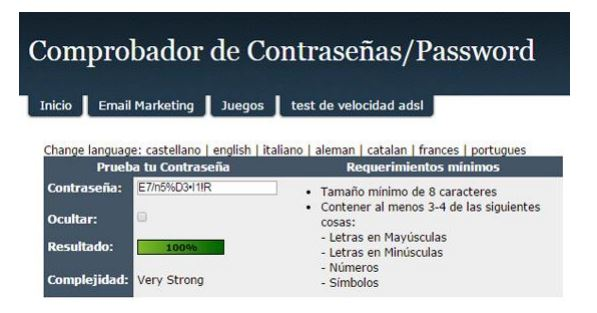
\includegraphics[width=7cm]{./Imagenes/login}
\end{center}	
\end{itemize}
\subsection{Preferencia de privilegios de usuario por privilegios de grupo}
\begin{itemize}
\item En ocasiones muchos usuarios reciben más privilegios sobre la base de datos de los que realmente
necesitan, lo que a la larga se puede convertir en un importante problema. Es recomendable modificar los
privilegios otorgados a los usuarios que estarán en contacto con la información con el fin de que no puedan
realizar modificaciones más allá de las autorizadas.
\item Si por ejemplo un usuario sólo realizará consultas a la base de datos pero no podrá modificar ningún
registro ni insertar nada nuevo, no tiene sentido que le ofrezcamos esos privilegios, ya que lo que estamos
haciendo es abrir una puerta para un eventual ataque.
\end{itemize}
\subsection{ Características de bases de datos innecesariamente habilitadas}
\begin{itemize}
\item Cada instalación de base de datos viene con una serie de paquetes o módulos adicionales de distintas
formas y tamaños que en muy pocas ocasiones todos ellos son utilizadas por las compañías, lo que las
convierten en una posible puerta de entrada para sufrir algún tipo de ataque si en esos paquetes se
descubre cualquier problema de seguridad. Para reducir riesgos, es recomendable que los usuarios
detecten esos paquetes que no se utilizan y se desactiven del servidor donde estén instalados. Esto no sólo
reduce los riesgos de ataques, sino que también simplifica la gestión de parches ya que únicamente será de
máxima urgencia actualizar aquellos que hagan referencia a un módulo que estemos utilizando.
\end{itemize}
\subsection{Desbordamiento de búfer}
\begin{itemize}
\item Se trata de otro de los medios favoritos utilizados por los piratas y que se dan por el exceso de información
que se puede llegar a enviar por medio del ingreso de información mediante el uso de formularios, es decir,
se recibe mucha más información de lo que la aplicación espera. Por poner un ejemplo, si se espera la
entrada de una cuenta bancaria que puede ocupar unos 25 caracteres y se permite la entrada de muchos
más caracteres desde ese campo, se podría dar este problema.
\end{itemize}
\subsection{Bases de datos sin actualizar}
\begin{itemize}
\item Como ocurre con cualquier tipo de aplicación que tengamos instalada en nuestra máquina, es necesario ir
actualizando la versión de nuestra base de datos con las últimas versiones lanzadas al mercado, ya que en
ellas se solucionan aquellos problemas de seguridad detectados, por lo que pondremos más barreras a los
posibles atacantes.
\begin{center}
	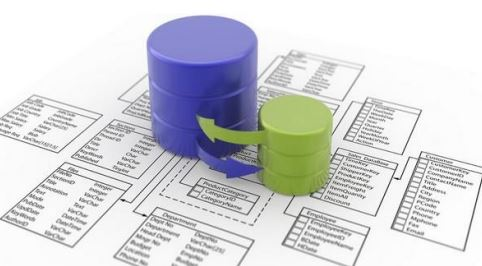
\includegraphics[width=7cm]{./Imagenes/bd}
\end{center}	
\item Para ello es muy importante estar informados de todos las noticias relacionadas con la base de datos que
estemos utilizando para saber en todo momento si algo nuevo ha sido lanzado al mercado que pueda
solucionar cualquier brecha de seguridad.
\end{itemize}
\subsection{ Datos sensibles sin cifrar}
\begin{itemize}
\item Aunque pueda ser algo obvio, a la hora de la verdad no todo el mundo cifra la información más importante
que se almacena en base de datos. Esto es una buena práctica para que en caso de hackeo, sea complicado
para el atacante poder recuperar esa información.
\item Por poner un ejemplo, las contraseñas de acceso a un sitio por parte de los usuarios podrían ser cifradas
utilizando el algoritmo MD5. De esta forma una contraseña del tipo “YUghd73j” en base de datos se
almacenaría con el siguiente valor “993e65b24451e0241617d6810849c824”. Como podéis ver, se trata de
un valor que poco o nada tiene que ver con el original.
\end{itemize}
\subsection{Injection SQL}
\begin{itemize}
\item Un ataque de este tipo puede dar acceso a alguien a una base de datos completa sin ningún tipo de
restricción, pudiendo llegar incluso a copiar y modificar los datos.
\item El lenguaje de consulta estructurado, o SQL, es un método para administrar bases de datos relacionales que se concibió por primera vez en la década de 1970. Desde entonces, se ha convertido en el estándar en los sistemas de gestión de bases de datos (DBMS) y se puede encontrar en innumerables organizaciones de todo el mundo.
\item SQLi funciona, al menos en la superficie, de una manera muy directa: un atacante envía una declaración SQL maliciosa en un campo que se puede rellenar que explota una vulnerabilidad en la implementación de SQL de la aplicación web.
\begin{center}
	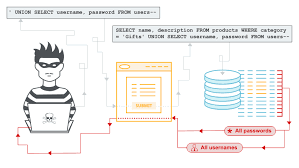
\includegraphics[width=7cm]{./Imagenes/1}
\end{center}	
\item Si tiene éxito, la declaración SQL maliciosa podría volcar todo el contenido de una base de datos, o seleccionar datos como registros de clientes, combinaciones de ID de empleado / contraseña, o cualquier otra cosa que contenga la base de datos seleccionada. SQLi también puede dar a un administrador de atacantes acceso a una base de datos, lo que les permite eliminar o modificar datos.
\begin{center}
	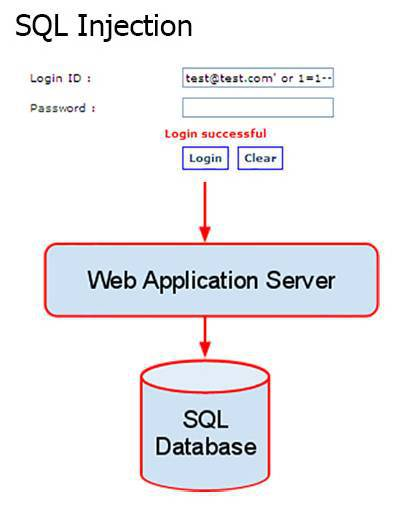
\includegraphics[width=7cm]{./Imagenes/2}
\end{center}	
	\item Los ataques de inyección SQL representan dos tercios de todos los ataques de aplicaciones web
Según los informes de Akamai, cuando se cuentan los ataques de inclusión de archivos locales, casi nueve de cada 10 ataques están relacionados con fallas de validación de entrada.
           \item Los ciberataques tienen varios vectores para acceder a las aplicaciones web, pero la inyección de SQL sigue siendo su opción más popular, según un nuevo análisis de datos de ataques.
           \item El ejercicio muestra que la inyección SQL (SQLi) ahora representa casi dos tercios   de todos Ataques de aplicaciones web. Eso se debe a la brusquedad de ataques en la  capa de aplicación web que SQLi representó hace solo dos años.
Los ataques de inclusión de archivos locales (LFI), que, como SQLi, también están habilitados por el hecho de que una aplicación web no haya validado correctamente los comentarios de los usuarios, representó otro 24.7 porciento de los ataques. En conjunto, los ataques SQLi y LFI representaron el 89.8 porciento de todos los ataques en la capa de aplicación .
- ¿Cuánta gente realmente entiende cómo escribir una aplicación que puede hablar de forma segura con la base de datos en el servidor?
 \item Pocos desarrolladores pueden entender la seguridad tan profundamente que una falla de seguridad realmente representaría un error para ellos.
\item  Los ataques SQLi clásicos son la forma más común y simple de SQLi.
\begin{center}
	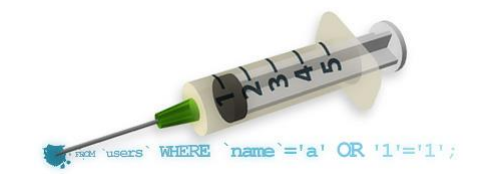
\includegraphics[width=7cm]{./Imagenes/3}
\end{center}	
\section{PROTEGERSE DE INYECCIÓN SQL}
\subsection {Asignacion de minimos privilegios}
\begin{itemize}
\item Debe tener los privilegios necesarios, ni mas ni menos.
\end{itemize}
\subsection {Validar todas las entradas}
\begin{itemize}
\item Especifique el tipo de dato de entrada, si son números,
asegúrese de que son solo números.
\end{itemize}
\subsection {Empleo de procedimientos almacenados}
\begin{itemize}
\item Utilizar procedimientos almacenados y aceptar los datos
del usuario como parámetros en lugar de comandos sql.
\end{itemize}
\subsection {Utilizar comillas dobles en lugar de simples}
\begin{itemize}
\item Puesto que las comillas simples finalizan las expresiones
SQL, y posibilitan la entrada de expresiones de más
potencia.
\end{itemize}
\end{itemize}
%-----------------------------------------------------------------
\section{Análisis}

\begin{itemize}
	\item Principalmente vemos la necesidad de conocer cada día mas el entorno de las bases de datos. Aprender de manera didáctica y autodidactica con mayor dedicación.

\item Es necesario conocer que la implementación del código debe estar bien estructurado para evitar algunas redundancias innecesarias.

\item Conocer las especificaciones que nos presenta cuando estructuramos las tablas de cada base de datos, realizando nuestro trabajo mas practico y sencillo.
\end{itemize}
%-----------------------------------------------------------------
\section{Conclusiones}

\begin{itemize}
	\item A través del desarrollo de las prácticas en laboratorio he conocido las ventajas de las bases de datos que se superponen a los sistemas de archivos del pasado, como sabemos todo evoluciona es así como el modelo relacional que implementa SQL, nos da una excelente herramienta en la administración, seguridad y fiabilidad de los datos.
	\item Aunque realizar la implementación de la seguridad más sofisticada no es tarea fácil, debemos hacer el esfuerzo de lograr que los datos estén completamente seguros para el bien de la información de las organizaciones, empresas, entre otros.
           \item Por lo tanto se sabe que conocer el proceso interno, la estructura he implementación de base de datos nos muestra la importancia que realizan en el mundo laboral, y como cada ente que las utiliza es dependiente de ellas.

\end{itemize}


% Bibliografia.
%-----------------------------------------------------------------

\bibliographystyle{plain}
\bibliography{Bibliografia}

\end{document}
